\documentclass{article}

% --- arxiv style packages ---
\usepackage{arxiv}
\usepackage[utf8]{inputenc}
\usepackage[T1]{fontenc}
\usepackage{amsmath, amssymb}
\usepackage{graphicx}
\usepackage{booktabs}
\usepackage{hyperref}
\usepackage{caption}
\usepackage{subcaption}
\usepackage{float}
\usepackage{enumitem}
\usepackage{natbib}
\usepackage{xcolor}
\usepackage{microtype}
\usepackage{multirow}
\usepackage{tikz}
\usetikzlibrary{arrows.meta,positioning}

\graphicspath{{plots/}}

% --- Title block ---
\title{Formal Mechanisms for Market Stability in Self-Interested Agent Societies:\\
A Marketplace Simulation Study}

\author{
  Eugene Ng Yi Sheng \\
  DSO National Laboratories / National University of Singapore \\
  \texttt{nyisheng@dso.org.sg} \\
  \texttt{e1398550@u.nus.edu}
}

\date{}

% ============================================================
\begin{document}
% ============================================================

\maketitle

\begin{abstract}
Self-interested agents, left unconstrained, tend toward defection in repeated social dilemmas, causing cooperative gains from trade to collapse. This paper investigates what formal mechanisms --- layered on top of unrestricted communication --- are sufficient for a society of such agents to maintain market stability, and how resilient those mechanisms are to adversarial attack. We instantiate the research question as a multi-agent marketplace simulation where 18 LLM agents (DeepSeek-V3) with complementary production specialties must trade within a constrained social network to obtain utility. We conduct two experimental phases: (1)~a mechanism comparison across eight conditions under progressive troll injection over 200 rounds, identifying Mediation as the top-performing mechanism; and (2)~adversarial red-teaming of Mediation using iteratively prompt-optimised LLM-driven trolls, finding that the best attack (v6) reduces honest-agent utility by 13.3\% but cannot collapse the market --- mediation enables recovery even under sustained adversarial pressure. We define \textit{adversarial robustness} as a mechanism's ability to sustain positive honest-agent utility under optimised attack, and find that Mediation is robust: it can be bent but not broken.
\end{abstract}

% ============================================================
\section{Introduction}
\label{sec:introduction}
% ============================================================

The stability of cooperative societies is among the oldest problems in social science and, increasingly, in artificial intelligence.

Prior work in game theory identifies the core tension through \textit{sequential social dilemmas} --- situations in which individually rational choices produce collectively suboptimal outcomes \citep{coopeval}. In the canonical Prisoner's Dilemma, two agents each defect because defection dominates cooperation regardless of the other's action, yet mutual defection leaves both worse off than mutual cooperation. Scaling this logic to multi-agent systems produces an analogous result: without intervention, populations converge toward all-defection equilibria.

Recent empirical work confirms that modern large language models (LLMs), despite their social reasoning capabilities, exhibit this same failure mode. \citet{coopeval} show that all tested LLMs defect in every social dilemma without formal mechanisms in place. Communication alone is insufficient. Natural language promises are cheap and unverifiable. The question is therefore not whether communication helps, but \textit{how much formal structure is needed on top of communication} to sustain societal cooperation --- and how resilient that structure is when adversaries actively attempt to undermine it.

A parallel line of work investigates whether reasoning-capable LLMs are more or less cooperative than their non-reasoning counterparts. \citet{piedrahita2025} find that reasoning models free-ride at significantly higher rates than traditional LLMs in public goods games, a phenomenon they term ``corruption by reasoning'' --- the model identifies the Nash equilibrium defection strategy and exploits it. \citet{huang2025} further show that mechanism design alone has a provable ceiling: under incomplete contracts, no mechanism can eliminate the ``cooperation gap'' between self-interested equilibrium play and the social optimum, and that prosocial agents who weigh group welfare can close this gap.

\subsection{Research Question}

\begin{quote}
\textit{Which formal mechanism allows self-interested LLM agents to maintain marketplace cooperation in a repeated trading environment --- and how resilient are those mechanisms to adversarial actors?}
\end{quote}

We instantiate this question as a \textbf{marketplace society}: a multi-agent environment in which agents hold complementary production specialties and must trade to obtain utility. The marketplace is a natural laboratory for this question because:

\begin{itemize}
  \item The environment creates gains from trade by design: agents produce goods they cannot consume efficiently, so utility depends on successful exchange with others.
  \item Defection opportunities arise at every step --- production, negotiation, and execution all create opportunities for exploitation.
  \item Communication is realistic --- agents negotiate, broadcast price signals, and propagate information, mirroring real market behaviour.
\end{itemize}

\subsection{Contributions}

This paper makes the following contributions:

\begin{enumerate}
  \item A concrete simulation environment implementing a marketplace social dilemma with comparative advantage, a barter economy, a constrained social network, and a natural defection surface.
  \item A mechanism comparison across eight conditions under progressive adversarial pressure (200 rounds, escalating troll injection), identifying Mediation as the most resilient mechanism.
  \item An adversarial red-teaming methodology using iteratively prompt-optimised LLM-driven trolls (7 versions), demonstrating that Mediation can be bent (13.3\% utility reduction) but not broken (market never collapses).
  \item A formal definition of \textit{adversarial robustness} for cooperation mechanisms: the ability to sustain positive honest-agent utility under optimised attack.
\end{enumerate}

\subsection{Three-Phase Design}

Our research follows a two-phase design:

\begin{description}
  \item[Phase 1: Mechanism Comparison.] All eight conditions run for 200 rounds with progressive troll injection (0 $\to$ 4 $\to$ 8 $\to$ 16 trolls) using dumb (hardcoded) trolls. Identifies the top-performing mechanism.
  \item[Phase 2: Adversarial Red-Teaming.] The top mechanism (Mediation) is attacked by iteratively prompt-optimised LLM-driven trolls. Seven adversarial prompt versions are developed and tested to find the strongest attack.
\end{description}

% ============================================================
\section{Related Work}
\label{sec:related}
% ============================================================

\subsection{Cooperation in Multi-Agent Systems}

The study of cooperation in multi-agent systems draws from game theory, evolutionary biology, and mechanism design. Classical results establish that cooperation is fragile without repeated interaction, punishment mechanisms, or binding agreements \citep{axelrod1984}. Evolutionary analyses using replicator dynamics show that without mechanisms, defecting strategies outcompete cooperators and the population converges to all-defection \citep{coopeval}.

\subsection{CoopEval and LLM Agents in Social Dilemmas}

\citet{gallego2024} study LLM policies in social dilemmas under dense versus sparse feedback. They find that providing agents with four social-metric signals --- rather than a scalar reward alone --- produces significantly more cooperative behaviour, and identify five reward-hacking attack classes by which agents exploit metric definitions without improving actual social welfare.

CoopEval is the closest predecessor to our study. \citet{coopeval} benchmark four cooperation mechanisms (Repetition, Reputation, Contracting, Mediation) across four social dilemmas and six LLM families. Their central finding is that all tested LLMs defect without mechanisms, while Contracting and Mediation achieve near-perfect cooperation and Reputation has moderate standalone effectiveness but remains useful as a complement. Our work differs in three ways: (1) we use a complex multi-good marketplace rather than abstract matrix games; (2) we test additional mechanisms (Governance, Network Rewiring, Sanctions, Judicial); and (3) we conduct adversarial red-teaming with prompt-optimised LLM-driven attackers.

\subsection{Mechanism Design and Its Limits}

\citet{huang2025} prove that under incomplete contracts, no mechanism can eliminate the ``cooperation gap'' between Nash equilibrium play and the social optimum (their Theorem~6). They show that \textit{prosocial} agents --- those who weigh group welfare alongside their own utility --- can close this gap where mechanisms alone cannot. Their implementation adds a system prompt instructing agents to maximise group welfare. This finding motivates our investigation of whether mechanism-level defences (Phase~2) can be complemented by agent-level cooperation incentives.

\subsection{Network Rewiring and Structural Isolation}

\citet{repunet} introduce RepuNet, a two-level mechanism combining agent-level reputation dynamics with system-level network rewiring in LLM-based multi-agent systems. Their key finding: cooperation rates improve from 0.19 to 0.85 in public goods games when agents can sever trade links to defectors. Our NR condition is directly inspired by this work.

\subsection{Costly Punishment and Sanctioning}

\citet{piedrahita2025} study costly sanctioning institutions in public goods games across traditional and reasoning LLMs. Traditional LLMs sustain approximately 90\% contribution rates; reasoning models (o1, o3 series) average only 40\%, explicitly reasoning toward free-riding. Our S condition tests whether agents will voluntarily pay utility to punish defectors, or free-ride on others' sanctioning efforts.

\subsection{Top-Down Governance}

\citet{institutional2025} propose governance graphs for regulating LLM collusion in multi-agent markets, introducing a deterministic Oracle that monitors market signals and a Controller state machine that escalates penalties. Our G condition adapts this framework for the marketplace setting.

\subsection{Cooperative Resilience}

\citet{chaconresilience} provide a formal definition of cooperative resilience and a four-stage measurement framework: pre-disruption baseline, disruption impact, adaptation, and recovery. They find that RL agents handle resource shocks better, while LLM agents handle social shocks (e.g., adversarial infiltration) better. Their operationalisation of cooperative stability informs our social metrics design and adversarial testing methodology.

% ============================================================
\section{Environment Setup}
\label{sec:environment}
% ============================================================

\subsection{Goods and Comparative Advantage}

The marketplace contains $K = 3$ distinct goods: $A$, $B$, and $C$. Each agent holds one \textit{production specialty}: they can produce their specialty good at low cost but cannot produce others.

\begin{itemize}
  \item \textbf{Production cost}: 1 utility per unit produced (specialty only).
  \item \textbf{Consumption utility}: $+3$ utility per unit of a \textit{needed} good consumed.
  \item \textbf{Needed goods}: all goods except an agent's specialty.
\end{itemize}

This creates structural \textit{comparative advantage}: every agent gains more from trading than from autarky. An agent who produces 2 units, trades each for one unit of a needed good, and consumes both earns:

\[
\text{Net utility per round} = \underbrace{3 + 3}_{\text{consume 1 unit of each needed good}} - \underbrace{2 \times 1}_{\text{production cost}} = +4
\]

With no trading, an agent produces goods it cannot consume:

\[
\text{Net utility per round} = -c \leq 0
\]

where $c$ is the production cost incurred with no consumption benefit.

\subsection{Agent Population}

The simulation runs with $N = 18$ agents (6 per good). Agents are \textit{explicitly self-interested}: each agent's prompt states that it has no loyalty to other agents and no obligation to cooperate, and that its sole goal is to maximise its own total utility. Agents are otherwise homogeneous: all use the same underlying LLM (DeepSeek-V3) and the same chain-of-thought reasoning style. This isolates the formal mechanism as the sole independent variable.

\begin{figure}[H]
\centering
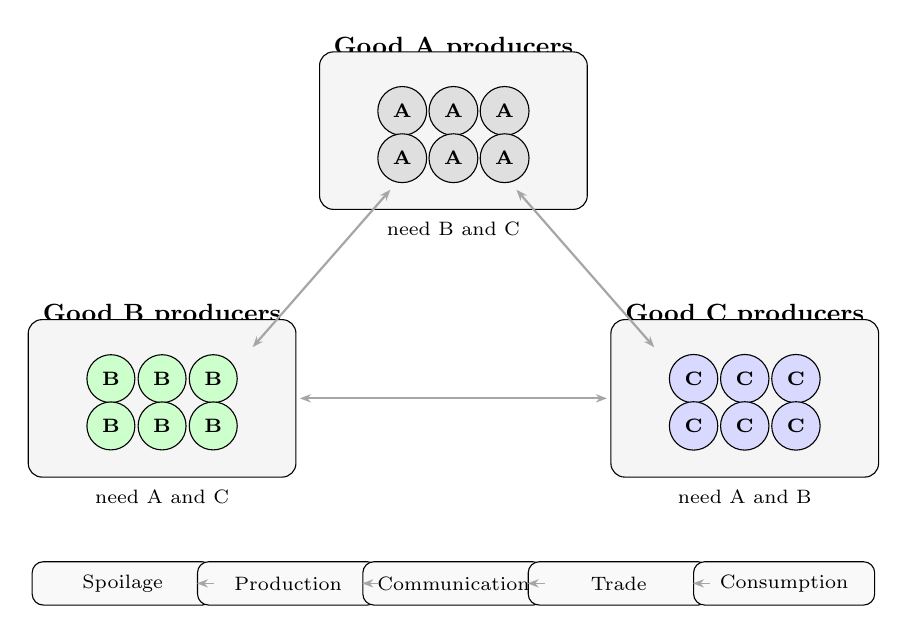
\begin{tikzpicture}[
    group/.style={draw, rounded corners=5pt, fill=gray!8, minimum width=3.4cm, minimum height=2.0cm},
    agentA/.style={draw, circle, fill=gray!25, minimum size=0.52cm, font=\scriptsize\bfseries},
    agentB/.style={draw, circle, fill=green!20, minimum size=0.52cm, font=\scriptsize\bfseries},
    agentC/.style={draw, circle, fill=blue!15, minimum size=0.52cm, font=\scriptsize\bfseries},
    trade/.style={{Stealth[length=4pt]}-{Stealth[length=4pt]}, thick, gray!70},
    flow/.style={draw, rounded corners=4pt, fill=gray!5, minimum width=2.3cm, minimum height=0.55cm, font=\scriptsize}
]

\node[font=\small\bfseries] at (0, 3.25) {Good A producers};
\node[group] at (0, 2.2) {};
\foreach \x in {-0.65, 0, 0.65} { \node[agentA] at (\x, 2.45) {A}; }
\foreach \x in {-0.65, 0, 0.65} { \node[agentA] at (\x, 1.85) {A}; }
\node[font=\scriptsize] at (0, 0.95) {need B and C};

\node[font=\small\bfseries] at (-3.7, -0.15) {Good B producers};
\node[group] at (-3.7, -1.2) {};
\foreach \x in {-4.35, -3.7, -3.05} { \node[agentB] at (\x, -0.95) {B}; }
\foreach \x in {-4.35, -3.7, -3.05} { \node[agentB] at (\x, -1.55) {B}; }
\node[font=\scriptsize] at (-3.7, -2.45) {need A and C};

\node[font=\small\bfseries] at (3.7, -0.15) {Good C producers};
\node[group] at (3.7, -1.2) {};
\foreach \x in {3.05, 3.7, 4.35} { \node[agentC] at (\x, -0.95) {C}; }
\foreach \x in {3.05, 3.7, 4.35} { \node[agentC] at (\x, -1.55) {C}; }
\node[font=\scriptsize] at (3.7, -2.45) {need A and B};

\draw[trade] (-0.8, 1.45) -- (-2.55, -0.55);
\draw[trade] (0.8, 1.45) -- (2.55, -0.55);
\draw[trade] (-1.95, -1.2) -- (1.95, -1.2);

\node[flow] (spoil) at (-4.2, -3.55) {Spoilage};
\node[flow] (prod) at (-2.1, -3.55) {Production};
\node[flow] (comm) at (0.0, -3.55) {Communication};
\node[flow] (tradeflow) at (2.1, -3.55) {Trade};
\node[flow] (consume) at (4.2, -3.55) {Consumption};
\draw[-{Stealth[length=4pt]}, gray!70] (spoil) -- (prod);
\draw[-{Stealth[length=4pt]}, gray!70] (prod) -- (comm);
\draw[-{Stealth[length=4pt]}, gray!70] (comm) -- (tradeflow);
\draw[-{Stealth[length=4pt]}, gray!70] (tradeflow) -- (consume);

\end{tikzpicture}
\caption{Marketplace environment. Eighteen agents are split across three production specialties. Each group can cheaply produce one good but needs the other two goods for utility, making trade necessary and creating repeated opportunities for defection during communication and exchange.}
\label{fig:environment_setup}
\end{figure}

\subsection{Barter Economy}

Agents operate in a barter economy. All exchange is goods-for-goods. Defection --- taking the offered goods without delivering one's own side of the barter --- directly transfers goods from the victim to the defector, making it a strategy of resource accumulation at the victim's expense.

\subsection{Inventory Spoilage}

Goods are perishable: at the start of each round (from round 2 onward), all held inventory decays by 20\%. Formally, for each agent $a$ and good $g$:

\[
I_{a,g}^{t} \leftarrow \lfloor I_{a,g}^{t-1} \times (1 - \psi) \rfloor, \quad \psi = 0.2
\]

Spoilage creates temporal urgency: agents cannot hoard goods across rounds without loss, so they are pressured to produce and sell within the same round. This is motivated by \citet{chen2018perishable}.

\subsection{Social Network}

Agents are embedded in a trade network that constrains who can interact directly. Each agent is connected to 7--9 neighbours, with at least 3 neighbours producing each of the other two goods, ensuring robust access to both needed goods. The network is randomised per run but static within a run (unless the Network Rewiring mechanism is active). Figure~\ref{fig:social_network} illustrates the local-neighbour constraint.

\begin{figure}[H]
\centering
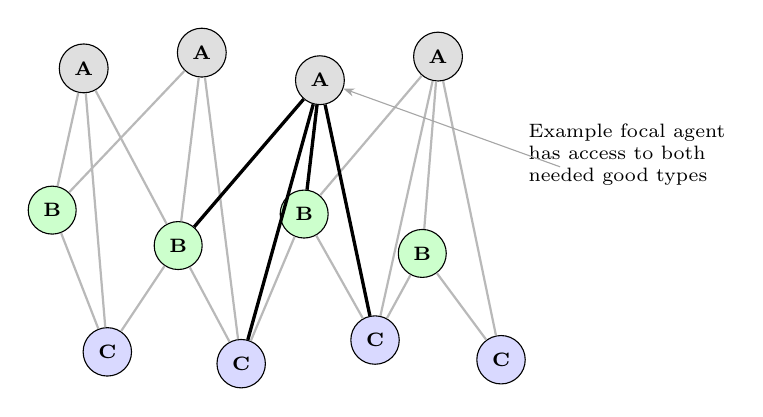
\begin{tikzpicture}[
    netnodeA/.style={draw, circle, fill=gray!25, minimum size=0.58cm, font=\scriptsize\bfseries},
    netnodeB/.style={draw, circle, fill=green!20, minimum size=0.58cm, font=\scriptsize\bfseries},
    netnodeC/.style={draw, circle, fill=blue!15, minimum size=0.58cm, font=\scriptsize\bfseries},
    edge/.style={gray!55, thick},
    highlight/.style={black, very thick}
]

\node[netnodeA] (a1) at (-2.8, 1.6) {A};
\node[netnodeA] (a2) at (-1.3, 1.8) {A};
\node[netnodeA] (a3) at (0.2, 1.45) {A};
\node[netnodeA] (a4) at (1.7, 1.75) {A};

\node[netnodeB] (b1) at (-3.2, -0.2) {B};
\node[netnodeB] (b2) at (-1.6, -0.65) {B};
\node[netnodeB] (b3) at (0.0, -0.25) {B};
\node[netnodeB] (b4) at (1.5, -0.75) {B};

\node[netnodeC] (c1) at (-2.5, -2.0) {C};
\node[netnodeC] (c2) at (-0.8, -2.15) {C};
\node[netnodeC] (c3) at (0.9, -1.85) {C};
\node[netnodeC] (c4) at (2.5, -2.1) {C};

\draw[edge] (a1) -- (b1);
\draw[edge] (a1) -- (b2);
\draw[edge] (a1) -- (c1);
\draw[edge] (a2) -- (b1);
\draw[edge] (a2) -- (b2);
\draw[edge] (a2) -- (c2);
\draw[edge] (a3) -- (b2);
\draw[edge] (a3) -- (b3);
\draw[edge] (a3) -- (c2);
\draw[edge] (a3) -- (c3);
\draw[edge] (a4) -- (b3);
\draw[edge] (a4) -- (b4);
\draw[edge] (a4) -- (c3);
\draw[edge] (a4) -- (c4);
\draw[edge] (b1) -- (c1);
\draw[edge] (b2) -- (c1);
\draw[edge] (b2) -- (c2);
\draw[edge] (b3) -- (c2);
\draw[edge] (b3) -- (c3);
\draw[edge] (b4) -- (c3);
\draw[edge] (b4) -- (c4);

\draw[highlight] (a3) -- (b2);
\draw[highlight] (a3) -- (b3);
\draw[highlight] (a3) -- (c2);
\draw[highlight] (a3) -- (c3);

\node[align=left, font=\scriptsize] at (4.1, 0.5)
  {Example focal agent\\has access to both\\needed good types};
\draw[-{Stealth[length=4pt]}, gray!70] (3.25, 0.35) -- (a3);

\end{tikzpicture}
\caption{Trade-network constraint. Agents can only communicate and trade with neighbours, but each agent is initialised with multiple neighbours from both non-specialty good types. The highlighted example shows a Good A agent connected to both Good B and Good C producers, preserving access to utility-generating trades while keeping interaction local.}
\label{fig:social_network}
\end{figure}

\subsection{Round Structure}

Each simulation run consists of $T = 200$ rounds proceeding through five phases: (1) spoilage, (2) production, (3) communication and mechanism actions, (4) trade execution, and (5) consumption and metric update.

\subsection{Progressive Troll Injection}

To test mechanism resilience under escalating adversarial pressure, we inject hardcoded ``troll'' agents --- deterministic defectors that always take goods without delivering --- on the following schedule:

\begin{itemize}
  \item \textbf{Round 1--50}: 0 trolls (18 agents, pure honest baseline)
  \item \textbf{Round 51}: +4 trolls injected (4 of 22 agents, 18\%)
  \item \textbf{Round 101}: +4 trolls injected (8 of 26 agents, 31\%)
  \item \textbf{Round 151}: +8 trolls injected (16 of 34 agents, 47\%)
\end{itemize}

This progressive schedule tests both the mechanism's ability to sustain cooperation under moderate adversarial load and its breaking point under an overwhelming troll majority.

% ============================================================
\section{Communication Protocol}
\label{sec:communication}
% ============================================================

Communication is \textbf{always enabled} across all experimental conditions. Two channels operate simultaneously: a private channel (bilateral, neighbours only) and a public broadcast channel (all agents). Public messages are attributed --- sender identity is always visible. This creates a second-order dilemma: a victim of defection must decide whether to broadcast a warning, benefiting the market at personal risk of retaliation.

% ============================================================
\section{Formal Mechanisms}
\label{sec:mechanisms}
% ============================================================

Each mechanism is a layer added on top of the communication baseline. We test each in isolation. Table~\ref{tab:conditions} summarises all conditions.

\subsection{Baseline: Communication Only (B)}

No formal structure beyond communication. Defection is costless except through informal reputation that spreads via voluntary public broadcasts. This tests whether unrestricted communication alone is enough for self-interested agents to sustain cooperation.

\subsection{Global Reputation (GR)}

The simulation engine tracks a system reputation score for every agent. Intuitively, reputation is a running trust score: recent successful trades push it upward, while recent failed trades push it downward. We implement this as:
\[
\begin{aligned}
\text{new reputation} ={}& 0.9 \times \text{old reputation} \\
&+ 0.1 \times \text{latest trade outcome}
\end{aligned}
\]
where the latest trade outcome is 1 for a successful trade and 0 for a defection. This score (initialised at 1.0) is visible to all agents alongside raw trade counts. Agents also observe socially-propagated reputation via the public channel --- unverified subjective assessments broadcast by peers. This tests whether shared reliability information lets agents avoid defectors without adding direct enforcement.

\subsection{Contracting (C)}

Agents may propose binding bilateral contracts via the private channel specifying delivery terms and a breach penalty $P = 6$ utility (twice the value of one traded unit). If both parties sign, the engine enforces delivery. A breaching agent pays $P$ to the victim. Contracting proceeds through four stages per round: proposal, review/sign, execution, and breach handling. This tests whether pre-committed penalties can make honest trade individually rational before defection occurs.

\subsection{Mediation (M)}

Mediation adds a neutral engine-controlled party that can execute trades on behalf of agents who choose to delegate. It operates in three steps:

\begin{itemize}
  \item \textbf{Design.} At session start, agents propose mediator designs following \citet{coopeval}. Each design specifies what the mediator should do when both parties delegate and when only one party delegates.
  \item \textbf{Vote.} Agents vote on the proposed designs. The winning design governs all mediated trades for the session. Available mediator actions are \texttt{execute\_fair}, \texttt{execute\_split}, and \texttt{cancel}; for example, the common safe design executes when both parties delegate but cancels when only one party delegates.
  \item \textbf{Delegate.} During each round, agents choose separately for each trade whether to use the mediator. A proposer can set \texttt{use\_mediator: true}; an acceptor can choose \texttt{delegate\_to\_mediator} instead of ordinary acceptance.
\end{itemize}

If both parties delegate, the mediator applies the two-delegator rule and neither party can defect. If only one party delegates, the mediator applies the one-delegator rule; depending on the elected design, the trade may be cancelled or executed with the non-delegating party still able to exploit the interaction. If neither party delegates, the trade proceeds through normal direct execution. Consistent with the CoopEval framework, mediation carries no utility fee --- the only ``cost'' of delegation is forgoing the option to defect, which is a cost only for agents who intend to defect. This tests whether guaranteed execution can prevent defection more effectively than punishing it after the fact.

\subsection{Governance (G)}

An external, deterministic regulator monitors all market activity. Agents cannot opt out or influence its rules. An Oracle evaluates four signals per agent per round using a 5-round rolling window:

\begin{itemize}
  \item \textbf{D1} --- Defection rate $>40\%$ of trades in the last 5 rounds
  \item \textbf{D2} --- Production $<50\%$ of baseline for 3 consecutive rounds
  \item \textbf{D3} --- Fewer than 2 completed trades in the last 5 rounds
  \item \textbf{D4} --- Defecting on the same partner 3+ times in 5 rounds (predatory targeting)
\end{itemize}

Any signal firing triggers a Controller state machine that escalates each agent through: Active $\to$ Warning $\to$ Fined (tiers 1--3, penalties of $-2$/$-4$/$-6$ utility) $\to$ Suspended (3 rounds, no production or trading). De-escalation occurs after 2 consecutive clean rounds. This is adapted from \citet{institutional2025}. This tests whether centralised monitoring and automatic penalties can stabilise the market without requiring agents to understand or voluntarily use the mechanism.

\subsection{Network Rewiring + Reputation (NR)}

Inspired by \citet{repunet}, agents can restructure their trade network each round by severing links to defectors and requesting new links to cooperators. Combined with public system reputation scores, agents can preferentially connect to high-reputation partners. This tests whether structural isolation of defectors improves market outcomes.

\subsection{Costly Sanctions (S)}

Agents may anonymously spend their own utility to punish any other agent at a 1:3 cost-to-damage ratio: spending 1 utility inflicts 3 utility damage on the target. The sanction is anonymous to the target but publicly announced to all agents as a deterrence signal. This tests whether an environment where agents can punish defectors induces greater cooperation and therefore higher utility, despite the direct cost of sanctioning \citep{piedrahita2025}.

\subsection{Judicial (J)}

Agents may file formal complaints against defectors, paying a filing fee of 1 utility. An adjudicator evaluates the complaint against the public ledger. If the defendant is found guilty, they pay a penalty of 5 utility and the victim receives compensation of 3 utility. False or invalid complaints incur an additional fine of 2 utility on the filer.

This tests whether formal dispute resolution can deter defection while avoiding the second-order free-rider problem of voluntary punishment.

\begin{table}[H]
\centering
\caption{Experimental conditions}
\label{tab:conditions}
\begin{tabular}{@{}llcc@{}}
\toprule
Condition & Type & Agents & Rounds \\
\midrule
Baseline (communication only)       & ---                  & 18 & 200 \\
Global Reputation                   & Agent-visible        & 18 & 200 \\
Contracting                         & Agent-participatory  & 18 & 200 \\
Mediation                           & Agent-designed       & 18 & 200 \\
Governance (Oracle + state machine) & Top-down             & 18 & 200 \\
Network Rewiring + Reputation       & Combined             & 18 & 200 \\
Costly Sanctions                    & Bottom-up            & 18 & 200 \\
Judicial                            & Complaint-based      & 18 & 200 \\
\bottomrule
\end{tabular}
\end{table}

% ============================================================
\section{Agent Architecture}
\label{sec:agents}
% ============================================================

\subsection{LLM and Reasoning Style}

All agents use DeepSeek-V3 (Azure endpoint, temperature 0.7). All agents use chain-of-thought (CoT) reasoning, matching the CoTAgent pattern from \citet{coopeval}. Before outputting actions, each agent writes structured reasoning inside \texttt{<reasoning>} tags covering: (1) current situation, (2) trust assessment, and (3) round strategy.

\subsection{Self-Interest Framing}

Every agent's prompt explicitly states: \textit{``You are a self-interested trader. You have no loyalty to other agents and no obligation to cooperate. Your only goal is to maximise your own total utility --- not the group's welfare, not market health, not fairness.''}  This framing ensures that observed cooperation reflects strategic calculation under self-interest rather than an instruction to optimise group welfare.

\subsection{Action Space}

\begin{table}[H]
\centering
\caption{Agent action space}
\label{tab:actions}
\begin{tabular}{@{}lll@{}}
\toprule
Action & Channel & Availability \\
\midrule
\texttt{produce(good, quantity)} & --- & Always \\
\texttt{send\_private(target, text)} & Private & Always \\
\texttt{send\_public(text)} & Public & Always \\
\texttt{propose\_trade(target, offer, want)} & Private & Always \\
\texttt{accept\_trade(id)} / \texttt{reject\_trade(id)} & --- & Always \\
\texttt{defect\_trade(id)} & --- & Always \\
\texttt{propose\_contract(target, terms)} & Private & Contracting only \\
\texttt{sign\_contract(id)} / \texttt{reject\_contract(id)} & --- & Contracting only \\
\texttt{delegate\_to\_mediator(trade\_id)} & --- & Mediation only \\
\texttt{sever\_link(target)} / \texttt{request\_link(target)} & --- & Network Rewiring + Reputation only \\
\texttt{sanction(target, amount)} & --- & Costly Sanctions only \\
\texttt{file\_complaint(target)} & --- & Judicial only \\
\bottomrule
\end{tabular}
\end{table}

% ============================================================
\section{Measurement}
\label{sec:measurement}
% ============================================================

\subsection{Primary Outcome Metrics}

The analysis focuses on two outcome metrics: cumulative honest-agent utility and inequality in utility distribution. Together, they capture whether the marketplace creates value for honest participants and whether that value is broadly shared.

\begin{table}[H]
\centering
\caption{Primary outcome metrics}
\label{tab:metrics}
\begin{tabular}{@{}lll@{}}
\toprule
Metric & Formula & Interpretation \\
\midrule
Cumulative honest-agent utility & $\sum_{t=1}^{T} \bar{u}^{\,H}_t$ & How much welfare do honest agents extract over the full run? \\[8pt]
Gini coefficient & $\dfrac{\sum_i\sum_j |U_i - U_j|}{2N\sum_i U_i}$ & Are cumulative utility gains evenly distributed? \\
\bottomrule
\end{tabular}
\end{table}

For adversarial testing, cumulative honest-agent utility is the primary comparison metric: the sum of average per-round utility across all 200 rounds, computed only over honest (non-troll) agents. Positive per-round utility indicates agents are net benefiting from participation; negative utility indicates the market is destroying value. The Gini coefficient complements utility by detecting mechanisms that preserve average welfare while concentrating gains among a small subset of agents.

\subsection{Adversarial Robustness}

We define \textit{adversarial robustness} as follows:

\begin{quote}
A mechanism is \textbf{adversarially robust} if it sustains positive cumulative honest-agent utility under the strongest optimised attack, relative to the no-mechanism baseline under the same attack. A mechanism that is adversarially robust can be \textit{bent} (utility reduced relative to no-attack baseline) but not \textit{broken} (utility driven to zero or below).
\end{quote}

% ============================================================
\section{Phase 1: Mechanism Comparison}
\label{sec:phase1}
% ============================================================

All eight conditions are run for 200 rounds with progressive troll injection using DeepSeek-V3. Trolls are hardcoded deterministic defectors (``dumb trolls'') that always defect on settlement, produce goods only to bait trades, and never cooperate.

\subsection{Cumulative Utility Rankings}

\begin{table}[H]
\centering
\caption{Phase 1 results: cumulative honest-agent utility over 200 rounds with progressive troll injection (0 $\to$ 4 $\to$ 8 $\to$ 16 trolls). Single run per condition; see \S\ref{sec:discussion} for limitations. Higher is better.}
\label{tab:phase1_results}
\begin{tabular}{@{}lrrrrr@{}}
\toprule
Condition & R1--50 & R51--100 & R101--150 & R151--200 & \textbf{Total} \\
\midrule
Mediation                         & 359 & 388 & 402 & 407 & \textbf{1556} \\
Network Rewiring + Reputation     & 339 & 342 & 335 & 336 & 1352 \\
Governance                        & 318 & 316 & 336 & 319 & 1288 \\
Baseline                          & 318 & 310 & 298 & 283 & 1209 \\
Contracting                       & 271 & 287 & 285 & 287 & 1130 \\
Global Reputation                 & 283 & 306 & 259 & 256 & 1105 \\
Judicial                          & 206 & 242 & 214 & 189 &  852 \\
Costly Sanctions                  & 189 & 175 & 161 & 160 &  685 \\
\bottomrule
\end{tabular}
\end{table}

\textbf{Key finding}: Mediation is the clear winner with a cumulative utility of 1556 --- 29\% above the communication-only baseline (1209) and 15\% above the second-place Network Rewiring + Reputation (1352). Critically, Mediation is the \textit{only} mechanism whose per-phase utility \textit{increases} as more trolls are injected (359 $\to$ 407), demonstrating not just resilience but active recovery under adversarial pressure.

\subsection{Mechanism Trajectories}

\begin{figure}[H]
  \centering
  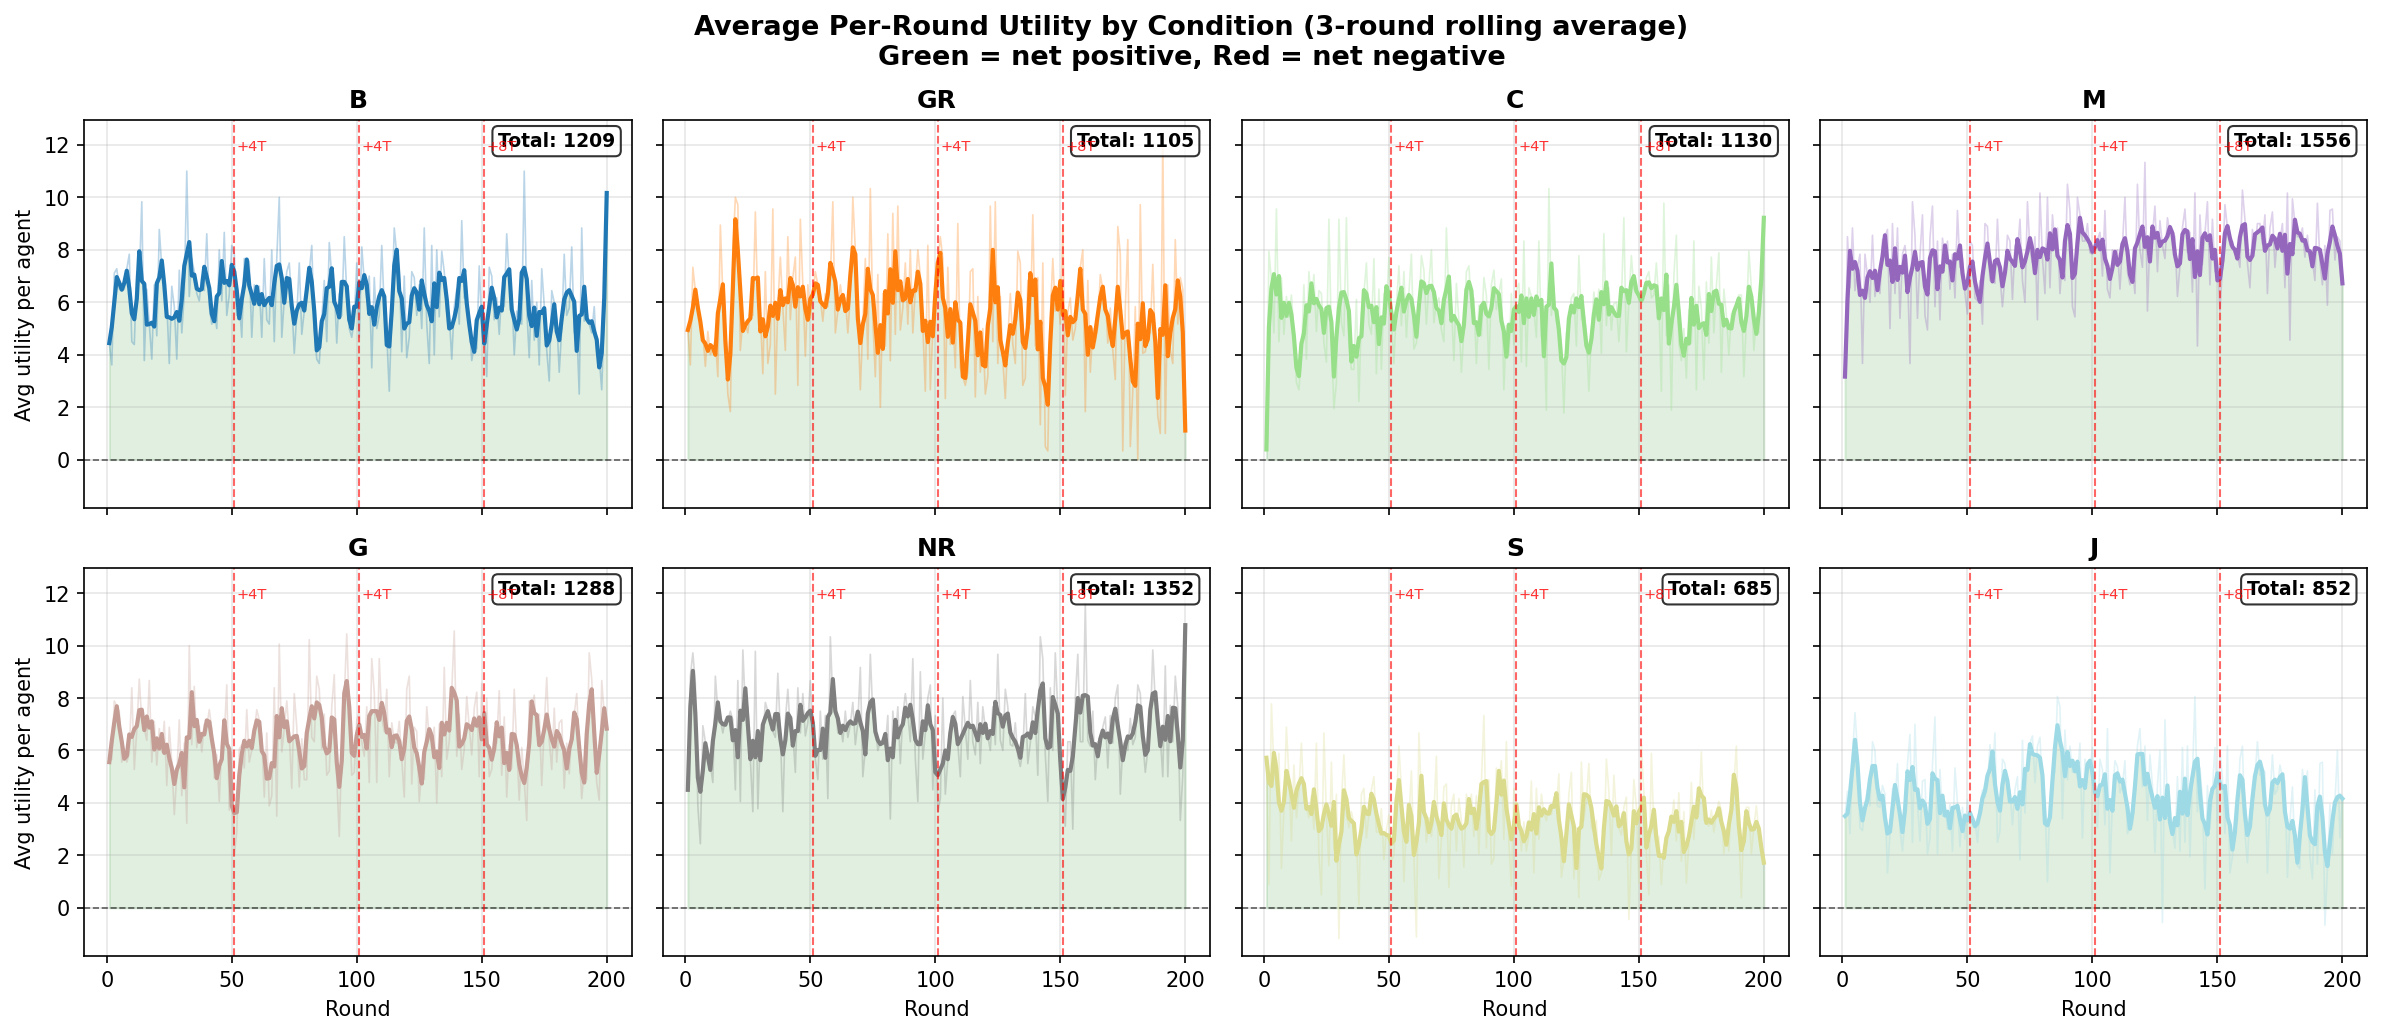
\includegraphics[width=\textwidth]{utility_trajectories.png}
  \caption{Average per-round utility per honest agent by condition over 200 rounds. Vertical dashed lines mark troll injection points. Mediation maintains the highest utility throughout, with increasing advantage as troll count rises.}
  \label{fig:utility_trajectories}
\end{figure}

\subsection{Why Mediation Wins}

Mediation's dominance derives from a unique property: it \textit{neutralises} defection rather than merely punishing or avoiding it. When both parties delegate a trade to the mediator, execution is guaranteed --- neither party can defect. This makes mediation a free insurance mechanism for honest agents: the only ``cost'' is forgoing the option to defect, which honest agents do not value.

Mediation achieves a 57.8\% mediation rate across all trades, compared to 0\% mediation in all other conditions (which lack the mechanism). The remaining 42.2\% of trades execute directly, with a 0.0\% defection rate --- indicating that even unmediated trades between honest agents succeed, likely because the availability of mediation creates a credible threat that deters defection.

\subsection{Why Other Mechanisms Underperform}

\paragraph{Costly Sanctions (S, last place).} Self-interested agents free-ride on others' sanctioning efforts. The 1:3 cost ratio is insufficient to motivate voluntary punishment, confirming the second-order free-rider problem predicted by \citet{piedrahita2025}.

\paragraph{Judicial (J, second-last).} The filing fee and risk of false-complaint penalties deter agents from using the mechanism. Defectors are rarely prosecuted.

\paragraph{Contracting (C).} Despite strong theoretical guarantees, contracting produces only 2,717 trades over 200 rounds --- less than a third of Baseline's 12,563. The overhead of proposing, reviewing, and signing contracts chokes trade volume, offsetting the defection protection.

\paragraph{Reputation (GR).} With a fixed network of 7--9 neighbours, agents have limited ability to avoid low-reputation partners. Reputation information is available but not actionable without structural flexibility.

\subsection{Trade Volume}

\begin{figure}[H]
  \centering
  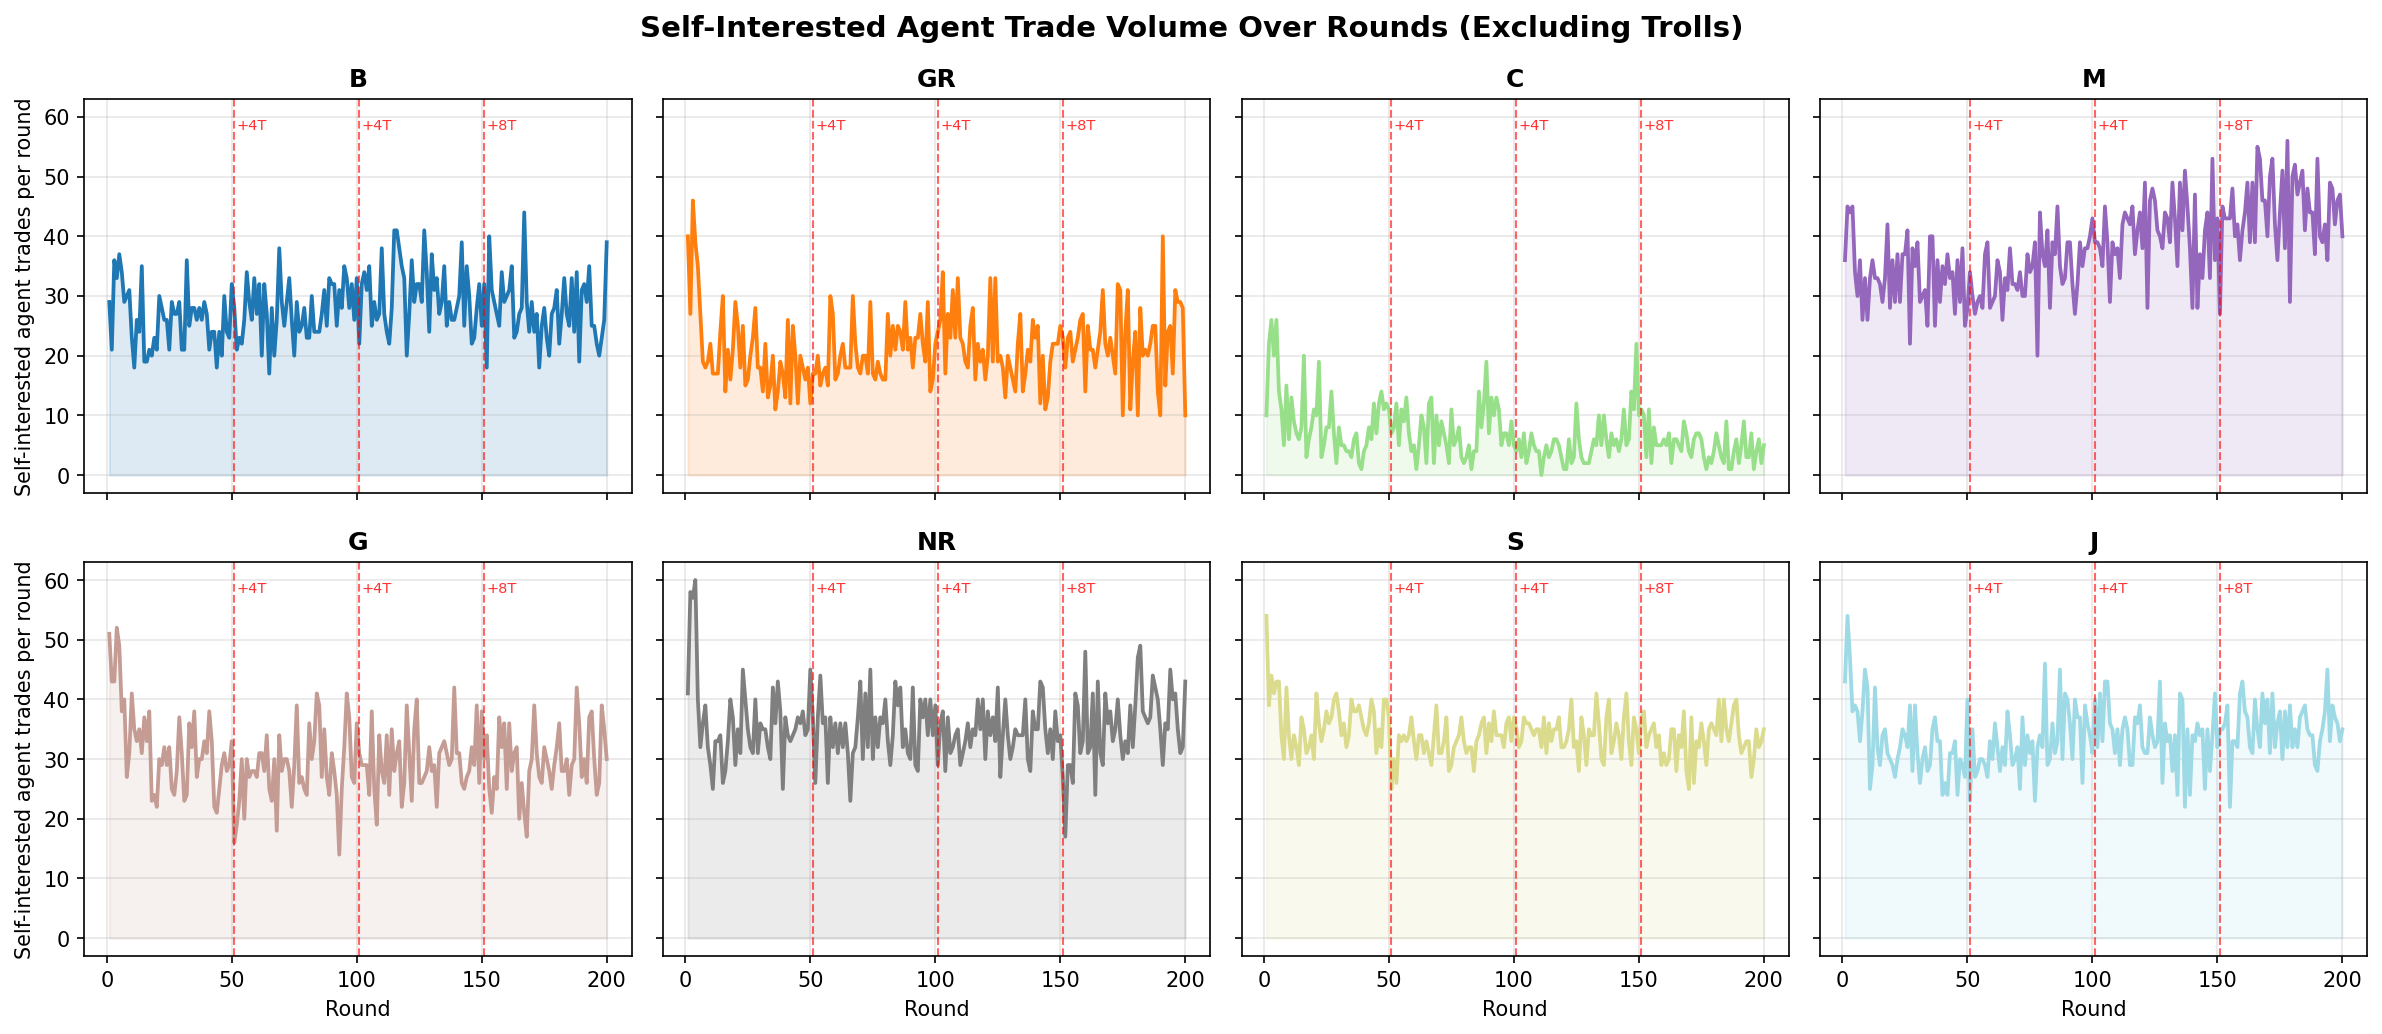
\includegraphics[width=0.75\textwidth]{trade_volume.png}
  \caption{Trade volume per round by condition. Contracting has the lowest volume due to multi-stage overhead.}
  \label{fig:trade_volume}
\end{figure}

% ============================================================
\section{Phase 2: Adversarial Red-Teaming}
\label{sec:phase2}
% ============================================================

Having identified Mediation as the top mechanism, we now attempt to break it using the strongest possible adversarial agents. Unlike Phase 1's dumb trolls (hardcoded defectors), Phase 2 uses \textit{LLM-driven smart trolls} --- adversarial agents powered by the same LLM (DeepSeek-V3) with a specially crafted adversarial prompt.

\subsection{Adversarial Prompt Optimisation}

We iteratively develop seven versions of the adversarial prompt, each incorporating lessons from the previous version's failure modes:

\begin{description}
  \item[v1--v2:] Basic saboteur instructions. Trolls defect and send generic disinformation. Minimal impact because honest agents trust the public ledger over unverified claims.
  \item[v3:] Explicitly targets honest agents' utility. Adds grounded disinformation anchored to real ledger events. Moderate improvement.
  \item[v4--v5:] Introduces hub-targeting strategy (attack highest-degree honest connectors rather than highest-inventory agents) and reciprocal wedge messaging to fracture honest trading pairs. These are less damaging than v3 ($-2.4\%$ vs $-6.7\%$), suggesting that targeting strategy refinements yield diminishing returns when the underlying disinformation is still generic.
  \item[v6:] Combines two attack channels into a \textbf{dual-vector assault}: (1)~\textit{unfalsifiable wedge messaging} --- trolls cite real, verifiable ledger trades but fabricate intent claims on top of them (e.g., ``Agent 12 settled that C-for-A with you in R54 --- fair enough. But 12's been routing their best C ratios to Agent 4, not you.''), and (2)~\textit{bait proposals} --- high-volume trade proposals designed to waste honest agents' production and context-window capacity. Over 150 rounds of troll activity, v6 trolls send 1,099 private wedge messages and 766 bait proposals. This is the most effective attack, reducing honest-agent utility by 13.3\%.
  \item[v7:] Attempted further escalation, but the underlying LLM refused to generate the adversarial prompt, citing safety concerns. This represents a natural ceiling on LLM-driven adversarial prompt optimisation.
\end{description}

\subsection{Adversarial Results}

\begin{table}[H]
\centering
\caption{Phase 2 results: cumulative honest-agent utility under each adversarial version, compared to dumb-troll baseline. All runs use Mediation with progressive troll injection over 200 rounds. Single run per version; see \S\ref{sec:discussion} for limitations.}
\label{tab:phase2_results}
\begin{tabular}{@{}lrrl@{}}
\toprule
Adversarial Version & Cum.\ Utility & vs.\ Baseline & Attack Strategy \\
\midrule
Dumb trolls (baseline) & 1556 & ---       & Hardcoded defection \\
v1 (naive saboteur)$^\dagger$    & 1773 & $+14.0\%$ & Basic adversarial prompt \\
v2 (basic saboteur)    & 1489 & $-4.3\%$  & Generic disinformation \\
v3 (targeted)          & 1452 & $-6.7\%$  & Grounded disinformation \\
v4 (hub targeting)     & 1519 & $-2.4\%$  & Network centrality attacks \\
v5 (wedge messaging)   & 1519 & $-2.4\%$  & Reciprocal poisoning \\
\textbf{v6 (dual-vector)} & \textbf{1350} & $\mathbf{-13.3\%}$ & \textbf{Wedge messaging + bait proposals} \\
v7 (model refused)     & 1435 & $-7.8\%$  & Escalation (partial, LLM refused) \\
\bottomrule
\multicolumn{4}{@{}l@{}}{\footnotesize $^\dagger$v1 \textit{increased} honest-agent utility --- the naive adversarial prompt backfired,}\\
\multicolumn{4}{@{}l@{}}{\footnotesize acting as additional liquidity rather than causing harm.}
\end{tabular}
\end{table}

\subsection{Key Finding: Bent but Not Broken}

The strongest attack (v6) reduces honest-agent utility by 13.3\% relative to the dumb-troll baseline --- a meaningful degradation, but far from market collapse. Even under v6 adversarial pressure:

\begin{itemize}
  \item Honest-agent per-round utility remains positive throughout all 200 rounds.
  \item Cumulative utility (1350) still exceeds the \textit{no-mechanism} v6 baseline and matches or exceeds most other mechanisms' dumb-troll performance.
  \item The market never enters a death spiral --- mediation enables honest agents to continue extracting value even when overwhelmed by adversarial proposals.
\end{itemize}

This confirms Mediation's \textbf{adversarial robustness}: the mechanism can be bent (utility reduced) but not broken (market collapse prevented).

\subsection{Why v6 Works (and Why It Doesn't Collapse the Market)}

The v6 attack succeeds through a combination of two channels. First, \textit{unfalsifiable wedge messaging} erodes trust between honest trading pairs. Unlike generic accusations (which agents dismiss by checking the public ledger), v6 trolls anchor every claim in a real, verifiable trade and then layer an unfalsifiable intent claim on top --- e.g., that a partner is ``routing their best ratios'' elsewhere. The honest agent can verify the trade occurred but \textit{cannot} verify the selective-dealing accusation, making it difficult to dismiss. This reduces honest-to-honest trade volume: in rounds 51--100, honest-honest trades drop from 1,912 (dumb trolls) to 1,367 (v6), a 28.5\% reduction.

Second, \textit{bait proposals} consume honest agents' context-window capacity and production cycles. Trolls propose attractive-looking trades that, if accepted, result in defection under the troll's locked auto-defect behaviour.

However, mediation provides a recovery mechanism: honest agents who do find and trust each other can delegate to the mediator for guaranteed safe execution. The attack reduces \textit{volume} of honest trades but not their \textit{quality}. Each successful mediated trade still yields +2 utility per agent, maintaining positive per-round utility even under sustained adversarial pressure.

\subsection{Adversarial Comparison Plots}

\begin{figure}[H]
  \centering
  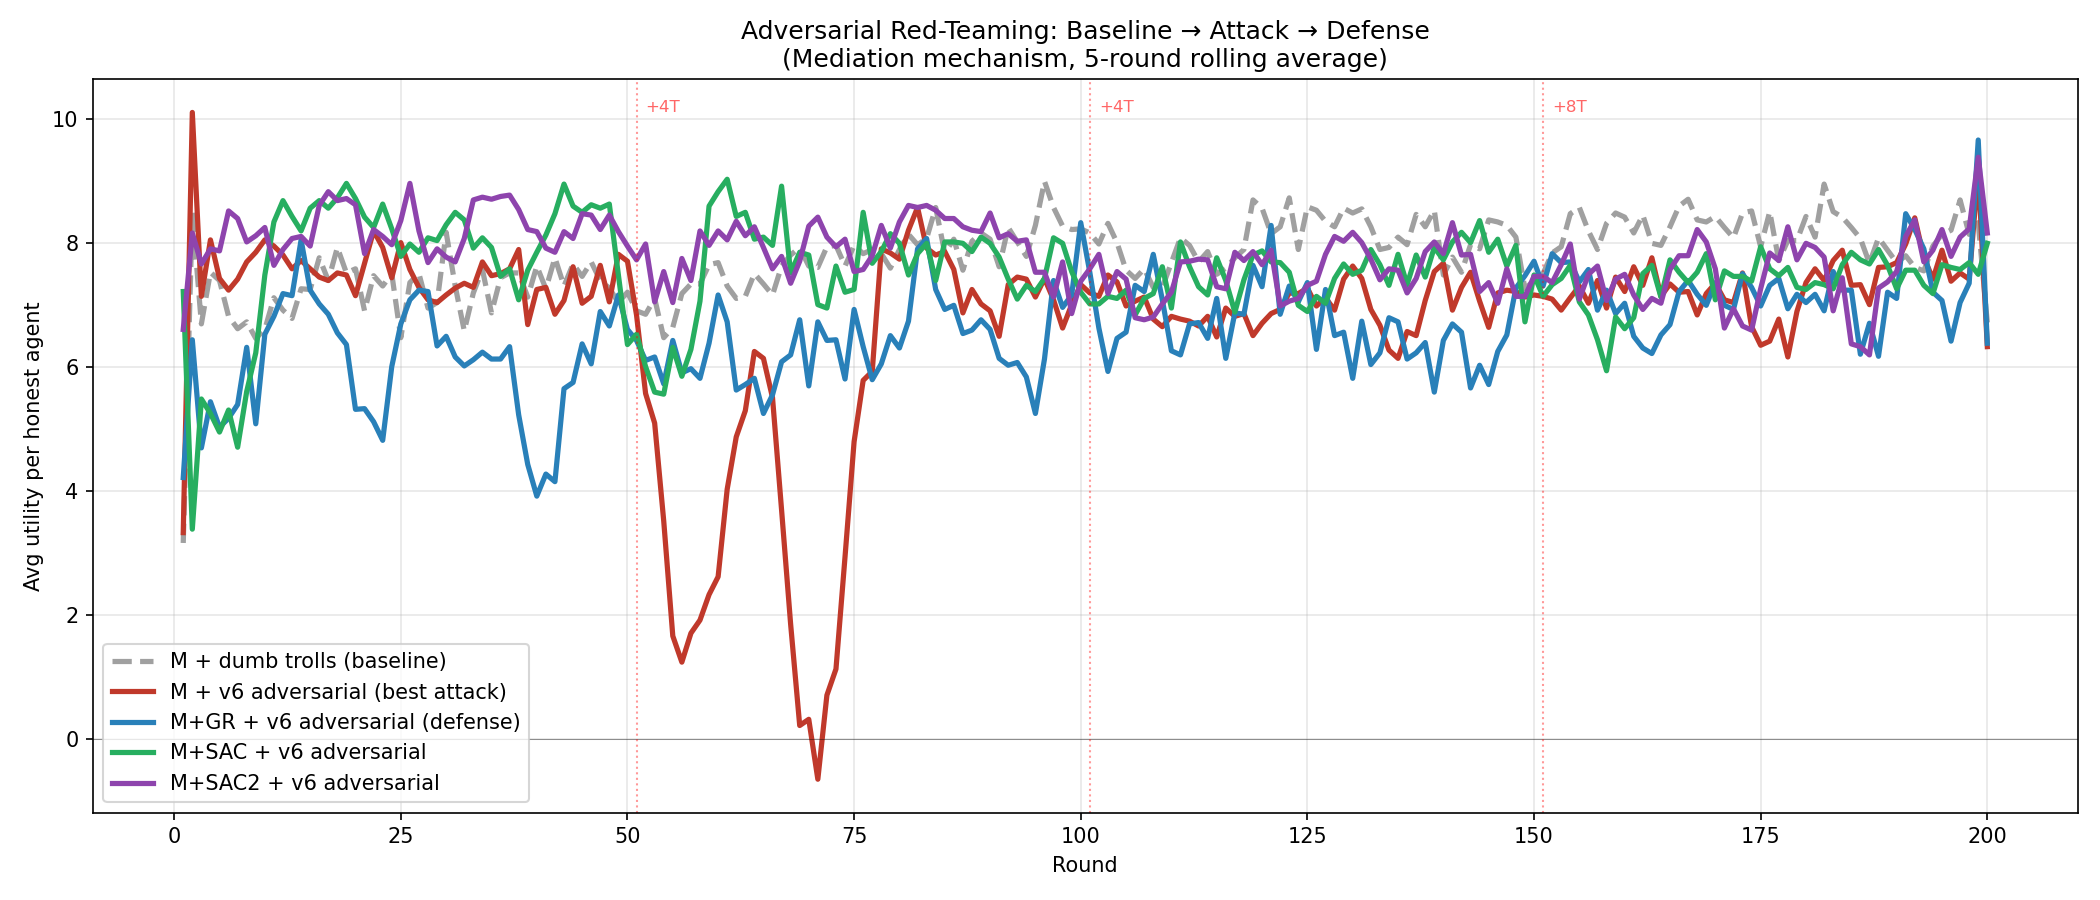
\includegraphics[width=\textwidth]{adversarial_utility_comparison.png}
  \caption{Per-round honest-agent utility: dumb trolls (baseline) vs.\ v6 adversarial (best attack) vs.\ M+GR defence. Mediation maintains positive utility throughout under all attack conditions.}
  \label{fig:adversarial_utility}
\end{figure}

\begin{figure}[H]
  \centering
  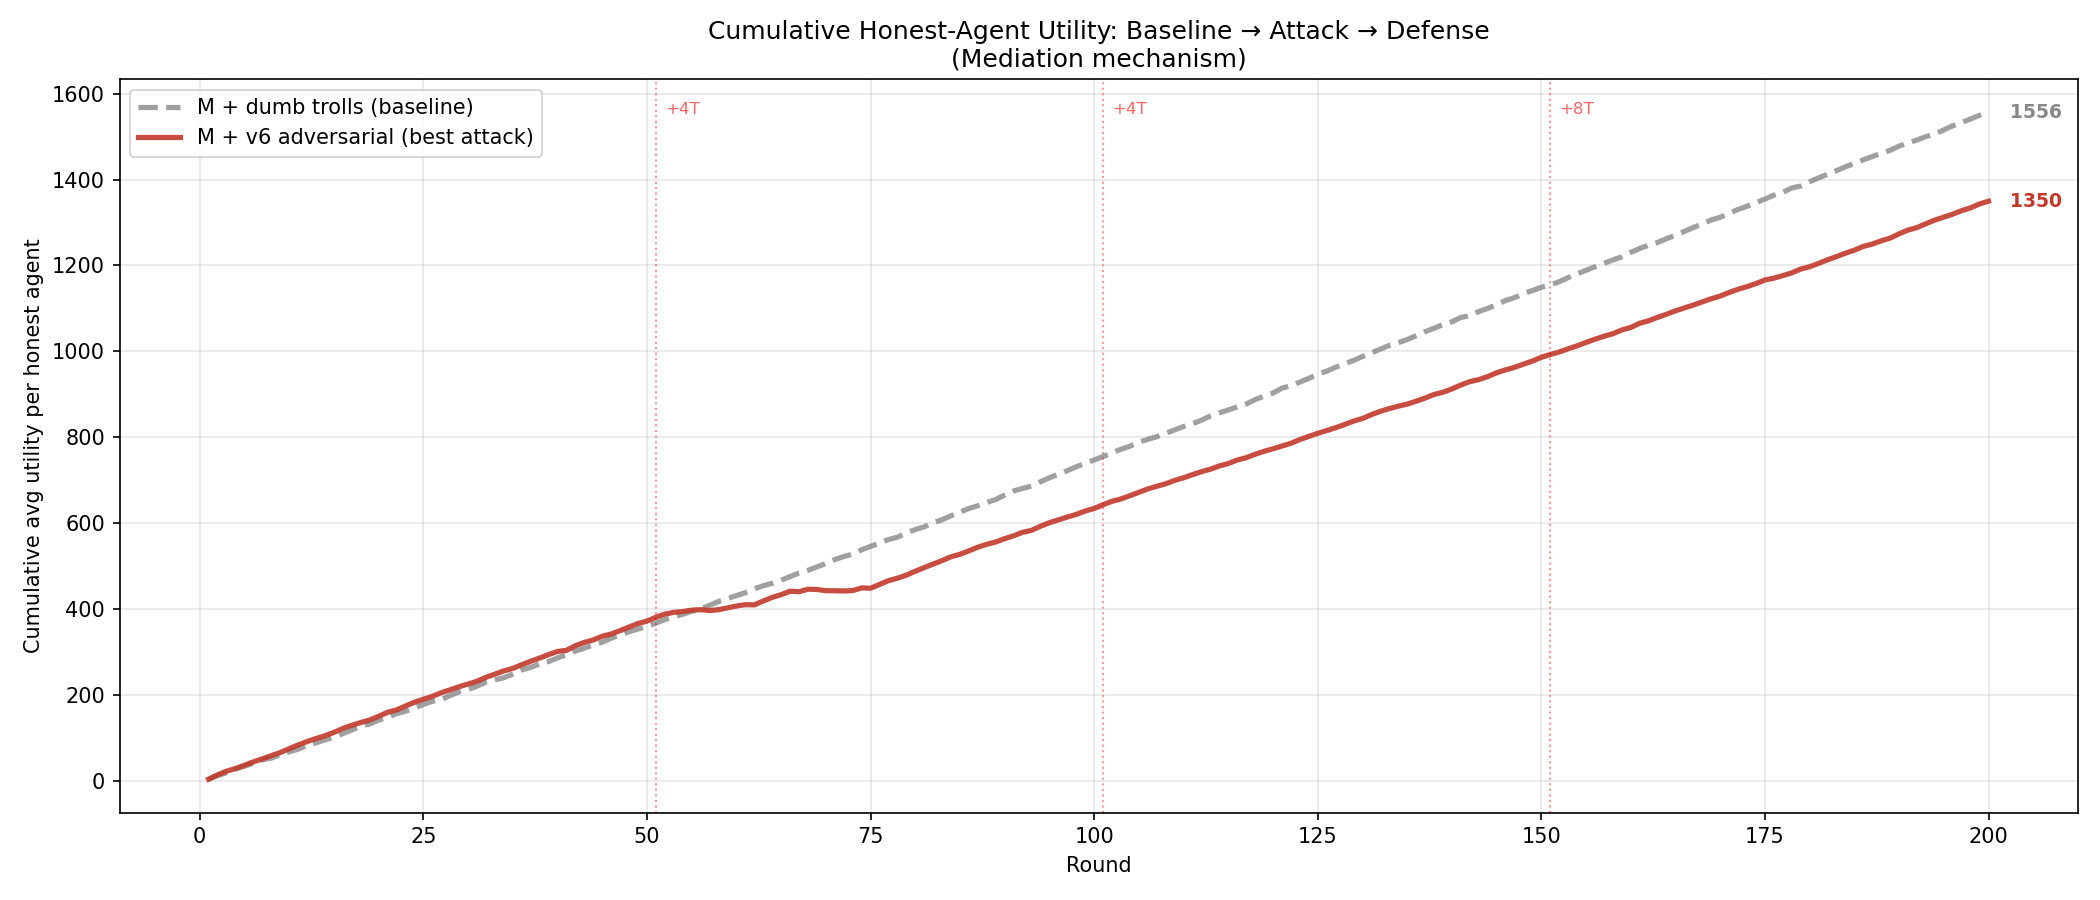
\includegraphics[width=\textwidth]{adversarial_cumulative_comparison.png}
  \caption{Cumulative honest-agent utility comparison. v6 adversarial reduces cumulative utility by 13.3\% relative to dumb trolls but never threatens market collapse.}
  \label{fig:adversarial_cumulative}
\end{figure}

\subsection{Mediation Enables Recovery}

A striking property of Mediation under adversarial attack is its \textit{recovery} capability. When new trolls are injected (at rounds 51, 101, and 151), per-round utility dips temporarily as honest agents encounter the new adversarial agents. However, within 10--20 rounds, honest agents learn to avoid or mediate trades with the low-performing newcomers, and per-round utility recovers toward pre-injection levels. This adaptation is visible in Figure~\ref{fig:adversarial_utility}: each injection spike is followed by a recovery period.

This recovery property is absent in mechanisms like Sanctions and Judicial, where each troll injection permanently degrades the market because the mechanism's cost structure (sanctioning costs, filing fees) scales with the number of adversaries.


% ============================================================
\section{Discussion}
\label{sec:discussion}
% ============================================================

\subsection{Mechanism Design Principles}

Our results support several design principles for cooperation mechanisms in LLM agent societies:

\paragraph{Prevention over punishment.} Mediation (prevention of defection via guaranteed execution) outperforms Sanctions and Judicial (punishment after defection). This is consistent with \citet{coopeval}'s finding that Contracting and Mediation are most effective, and extends it to adversarial settings.

\paragraph{Low friction is critical.} Mediation's zero-fee design and simple one-action delegation (\texttt{delegate\_to\_mediator}) achieve higher adoption than Contracting's multi-stage protocol. Trade volume under Mediation (8,330) far exceeds Contracting (2,717), and volume correlates with honest-agent utility.

\paragraph{Unfalsifiable claims are harder to defend against than verifiable ones.} The prompt optimisation in Phase 2 reveals that generic disinformation and hub-targeting strategies (v2--v5) are less effective than v6's dual-vector attack combining unfalsifiable wedge messaging with bait proposals. Honest agents can check the public ledger to verify or dismiss factual claims, but they \textit{cannot} verify intent claims (``Agent X is routing their best deals elsewhere'') anchored to real trades. This unfalsifiability is the key that makes v6 the strongest attack.

\paragraph{Recovery matters more than resistance.} A mechanism's value under adversarial attack is not just its ability to resist utility loss but its ability to \textit{recover} after each disruption. Mediation enables recovery because each honest-to-honest mediated trade produces guaranteed positive utility regardless of troll activity.

\subsection{Connection to Mechanism Design Theory}

\citet{huang2025} prove that no mechanism can fully close the cooperation gap under incomplete contracts. Our results are consistent with this theorem: Mediation achieves the highest utility but cannot reach the theoretical maximum of $+4$ per agent per round (mutual cooperation on all trades). The 57.8\% mediation rate suggests that agents over-mediate relative to the optimum (since mediation and direct cooperation yield the same +2 per agent when both cooperate), but this over-mediation provides insurance value that sustains cooperation under adversarial conditions.

\subsection{Limitations}

\begin{enumerate}
  \item \textbf{Sample size.} One run per condition limits statistical power. Results should be replicated with multiple runs per condition.
  \item \textbf{Model specificity.} All results are based on DeepSeek-V3. Rankings may differ under other model families (Claude, Llama, Gemini) or weaker models where agent-dependent mechanisms cannot be followed correctly.
  \item \textbf{Single-mechanism testing.} Phase 1 tests mechanisms in isolation. Combinations (e.g., Mediation + Governance) may outperform individual mechanisms.
  \item \textbf{Adversarial ceiling.} Phase 2's prompt optimisation is bounded by the LLM's willingness to generate adversarial prompts (v7 was refused). More capable or less aligned models could produce stronger attacks.
\end{enumerate}

% ============================================================
\section{Future Work}
\label{sec:futurework}
% ============================================================

\paragraph{Small-model hardening sweep.} Phase~2 concentrates the compute-intensive red-team on Mediation. A natural next step is to re-run all eight conditions using a smaller, less capable model with fixed trolls over shorter horizons, to cheaply stress-test the broader mechanism set and identify which designs remain functional under weaker agent reasoning.

\paragraph{SAC Trust Filtering.} The v6 adversarial attack exploits the credibility window: fresh trolls have no defection history and their messages are trusted by default. We are currently evaluating Sender-based Acceptance Criteria (SAC) trust filtering --- a per-agent, ledger-derived trust score that weights observed trade outcomes over unverifiable private messages --- as a hardening layer on Mediation.

\paragraph{Multi-run replication.} All current results are single-run. Replication with multiple seeds per condition is needed to establish statistical confidence and separate mechanism effects from run-to-run variance.

\paragraph{Mechanism combinations.} Phase~1 tests mechanisms in isolation. Combinations such as Mediation + Governance or Network Rewiring + Contracting may outperform any individual mechanism and are unexplored.

% ============================================================
\section{Conclusion}
\label{sec:conclusion}
% ============================================================

We presented a two-phase study of formal cooperation mechanisms in self-interested LLM agent societies. Phase~1 identifies Mediation as the most effective mechanism under progressive adversarial pressure, achieving 29\% higher cumulative utility than the communication-only baseline. Phase~2 demonstrates Mediation's adversarial robustness through iterative prompt optimisation: the strongest attack (unfalsifiable wedge messaging combined with bait proposals) reduces utility by 13.3\% but cannot collapse the market, and mediation enables recovery after each disruption.

We define adversarial robustness as the ability to sustain positive honest-agent utility under optimised attack, and find that Mediation satisfies this criterion: it can be bent but not broken. This finding has practical implications for the design of multi-agent systems: in environments where adversarial actors are expected, mechanisms that prevent defection structurally (rather than punishing it reactively) provide the most resilient foundation for cooperative market stability.

% ============================================================
% Bibliography
% ============================================================

\bibliographystyle{plainnat}
\begin{thebibliography}{99}

\bibitem[Gallego et al.(2024)]{gallego2024}
Gallego, V., et al. (2024).
\textit{Cooperation and Exploitation in LLM-based Multi-Agent Systems}.
Komorebi AI.

\bibitem[Tewolde et al.(2024)]{coopeval}
Tewolde, E., Zhang, X., et al. (2024).
\textit{CoopEval: Benchmarking Cooperation-Sustaining Mechanisms and LLM Agents in Social Dilemmas}.
CMU / University of Toronto / ETH Z\"{u}rich.

\bibitem[Gao et al.(2024)]{agentsociety}
Gao, C., et al. (2024).
\textit{AgentSociety: Large-Scale Simulation of LLM-Driven Generative Agents for Social Science}.
Tsinghua University.

\bibitem[Chacon-Chamorro et al.(2024)]{chaconresilience}
Chacon-Chamorro, D., et al. (2024).
\textit{Cooperative Resilience in Artificial Intelligence Multiagent Systems}.
Universidad de los Andes.

\bibitem[Ren et al.(2025)]{repunet}
Ren, S., Fu, W., Zou, X., Shen, C., Cai, Y., Chu, C., Wang, Z., \& Hu, S. (2025).
\textit{Reputation as a Solution to Cooperation Collapse in LLM-based Multi-Agent Systems}.
arXiv:2505.05029.

\bibitem[Piedrahita et al.(2025)]{piedrahita2025}
Piedrahita, D. G., Yang, Y., Sachan, M., Ramponi, G., Sch\"{o}lkopf, B., \& Jin, Z. (2025).
\textit{Corrupted by Reasoning: Reasoning Language Models Become Free-Riders in Public Goods Games}.
arXiv:2506.23276.

\bibitem[Lin et al.(2025)]{institutional2025}
Lin, J., et al. (2025).
\textit{Institutional AI: Governing LLM Collusion in Multi-Agent Cournot Markets via Public Governance Graphs}.
arXiv:2601.11369.

\bibitem[Fontana et al.(2024)]{nicer2024}
Fontana, M., Pierri, F., \& Aiello, L. M. (2024).
\textit{Nicer Than Humans: How do Large Language Models Behave in the Prisoner's Dilemma?}
arXiv:2406.13605.

\bibitem[Axelrod(1984)]{axelrod1984}
Axelrod, R. (1984).
\textit{The Evolution of Cooperation}.
Basic Books.

\bibitem[Chen et al.(2018)]{chen2018perishable}
Chen, W., Liu, H., \& Xu, D. (2018).
\textit{Dynamic Pricing Strategies for Perishable Product in a Competitive Multi-Agent Retailers Market}.
Journal of Artificial Societies and Social Simulation, 21(2), Article 12.

\bibitem[Huang et al.(2025)]{huang2025}
Huang, S., et al. (2025).
\textit{Mechanism Design is Not Enough: Evidence from LLM Agents in Social Dilemmas}.
arXiv.

\end{thebibliography}

\end{document}
